\documentclass[conference]{IEEEtran}
\IEEEoverridecommandlockouts
% The preceding line is only needed to identify funding in the first footnote. If that is unneeded, please comment it out.
\usepackage{cite}
\usepackage{amsmath,amssymb,amsfonts}
\usepackage{algorithmic}
\usepackage{graphicx}
\usepackage{textcomp}
\usepackage{xcolor}
\usepackage{cleveref}
\def\BibTeX{{\rm B\kern-.05em{\sc i\kern-.025em b}\kern-.08em
    T\kern-.1667em\lower.7ex\hbox{E}\kern-.125emX}}


\DeclareMathOperator{\atantwo}{atan2}



\begin{document}

\title{Aarhus University MSc Course Project  \\ Control of Mobile Robots (AY 2019-20)}

\author{\IEEEauthorblockN{S. L. Skovgaard}
\IEEEauthorblockA{\textit{dept. of Engineering (of Aff.)} \\
\textit{Aarhus Unitversity (of Aff.)}\\
Aarhus, Denmark \\
201401682@post.au.dk}}

\maketitle

\begin{abstract}

The article will document how to develop control software for UAV's and simulate the controller using the popular Gazebo software. 	

\end{abstract}

\section{Introduction}
The main focus of this paper will be to explain and document the control software used to control a UAV robot. The software makes use of the robot operation system ROS. The paper will explain theory, code, simulation and results with accompanying figures and plots. The main objective of this project is to get a UAV to autonomously navigate to four coordinate-points.

\section{Theory}\label{theory}
\subsection{The Robot Operating System}
In order to develop software for robots in a structured and easy way, the robot operating system(ROS)\cite{ros} has been used for this project. ROS is based upon the subscriber-publisher pattern where nodes is able to publish data as topics and subscribe to specific topics. In this project a node has been developed that is a subscriber and publisher which enables the node to: gather data, make calculations using this data and the publish new data. Furthermore a another node has been made solely for the purpose of gathering data and displaying this data using different plots.

\subsection{Parrot Bebop2 drone}
In order for the UAV to be able navigate to the given coordinates, a closed-loop control algorithm has to be developed in this case a p-controller is used to control the UAV. The UAV is a Parrot Bebob2 and is controlled using the package "bebop\_autonomy". By using this package it is possible to send velocity and angular velocity commands to a ROS topic and thereby control the speed and orientation of the drone. 

The p-controller developed in this project works by calculating the distance from the UAV to the currently active goal and use this as the error for the controller. A constant is multiplied to the error and the product of this will be used to set the velocity of the UAV.

\subsection{Inertial frame and body frame}
Two important aspects of UAV control software is the \textit{inertial frame} and \textit{body frame}.

\textbf{Intertial frame:} is an earth-fixed coordinates system. It is also sometimes described as a  north-east-down or NED reference frame, where north is the inertial x direction, east is the inertial y direction and down is the inertial z direction\cite{book}. 

\textbf{Body frame: } is a coordinates system fixed to the body of the vehicle with its origin at the center of mass, x-axis pointing along the fuselage reference line, z-axis pointing down perpendicular to x and y-axis. The coordinate system rotates with the vehicle. 

As a task for this project the Bebop2 drone must navigate between the goal-coordinates with different fixed yaw angles. In order for the controller to work as intended a transformation of the inertial-frame coordinates system to the body frame coordinate-system is needed. This is done by rotating inertial frame three times. First around z-axis(yaw), then y-axis(pitch) of the new coordinate system and lastly around the x-axis(roll).  

\subsection{Gazebo}
Gazebo is simulation environment that works together with ROS and is therefore suitable as a simulation tool for this project. Parrot provides the Bebop2 UAV as a downloadable package for Gazebo and this package is used for this project.

\section{Python code}
The code used for this project is built using the rospy package which is a Python library. Roscpp is also available if C++ is preferred. 

As mentioned earlier in this article, ROS makes use of the publisher/subscribre pattern. A single node containing several classes have been made for this project. The classes are: p-controller, takeoff and plot\_maker. 

\textbf{P-controller:} The responsibility of p-controller is handle the calculations and navigation of the UAV. The error or the euclidean distance to the goal-coordinates is calculated by first calculating the distance in the x-plane then the y-plane and lastly the z-plane. This results in three different distances which all are used as the error in each axis. The error are multiplied a constant \textit{kp} and lastly the product of this is used to set the velocity in each direction, x, y and z.

\textbf{Takeoff:} As the name suggests this class handles the takeoff. It's a simple class that makes sure the drone has performed a complete takeoff sequence and when this is done it no longer has any responsibility. 

\textbf{Plot\_maker:} This class subscribes to the same topic as the p-controller class, /bebob/odom. It stores all values obtained from odometry and when the UAV has been to all goal-coordinates, displays a number of plots which will be discussed later in the article. 


One task for this project is to navigate to the four goals with a set yaw angle, this however haven't been completed here as the author has no idea how the rotation matrices are supposed to be programmed. 

\section{Results and discussion}


\subsection{Simulation results}
To verify that the controller behaves as expected and to ensure that the drone will not crash when testing in real life, the controller has been tested in simulation first. The behaviour should be more or less the same when testing in a real world scenario. The simulation tests covers both the hovering and waypoint scenario however, only the waypoint scenario will be shown in this report. The drone used for the simulation as well as in the real world is the Parrot bebop2 UAV.

The controller coefficients are set to: Kp = 0.1, Ki = 0.01 and Kd = 0.1 as these values resulted in a reasonably quick and stable controller. On \cref{fig:sim_pos} the x, y and z position of the drone can be seen. It shows nicely how the drone goes to each waypoint in a controlled manner with a acceptable level of overshoot.  

\begin{figure}[hbtp]
	\centering
	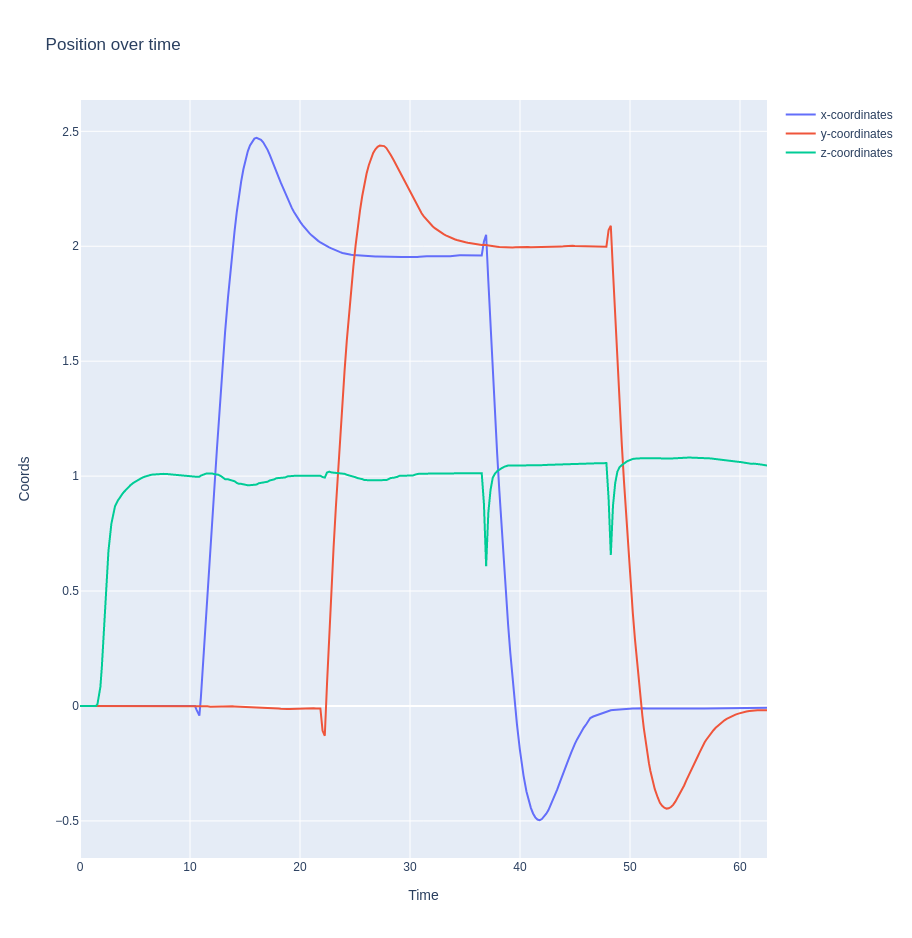
\includegraphics[width=1.0\linewidth]{images/task2_sim_pos.png}
	\caption{x, y and z coordinates of the drone in simulation. (Kp = 0.1, Ki = 0.01, Kd = 0.1)}
	\label{fig:sim_pos}
\end{figure}

Another way to visualize the simulation is using the program rviz which makes is possible to display the orientation as well as the position in 3D space. This can be seen on \cref{fig:sim_rviz}. On this figure it is also apparent that the yaw angle is constant for the drone at all times. 
After verifying that the drone is flying as intended in simulation real world testing can begin.

\begin{figure}[hbtp]
	\centering
	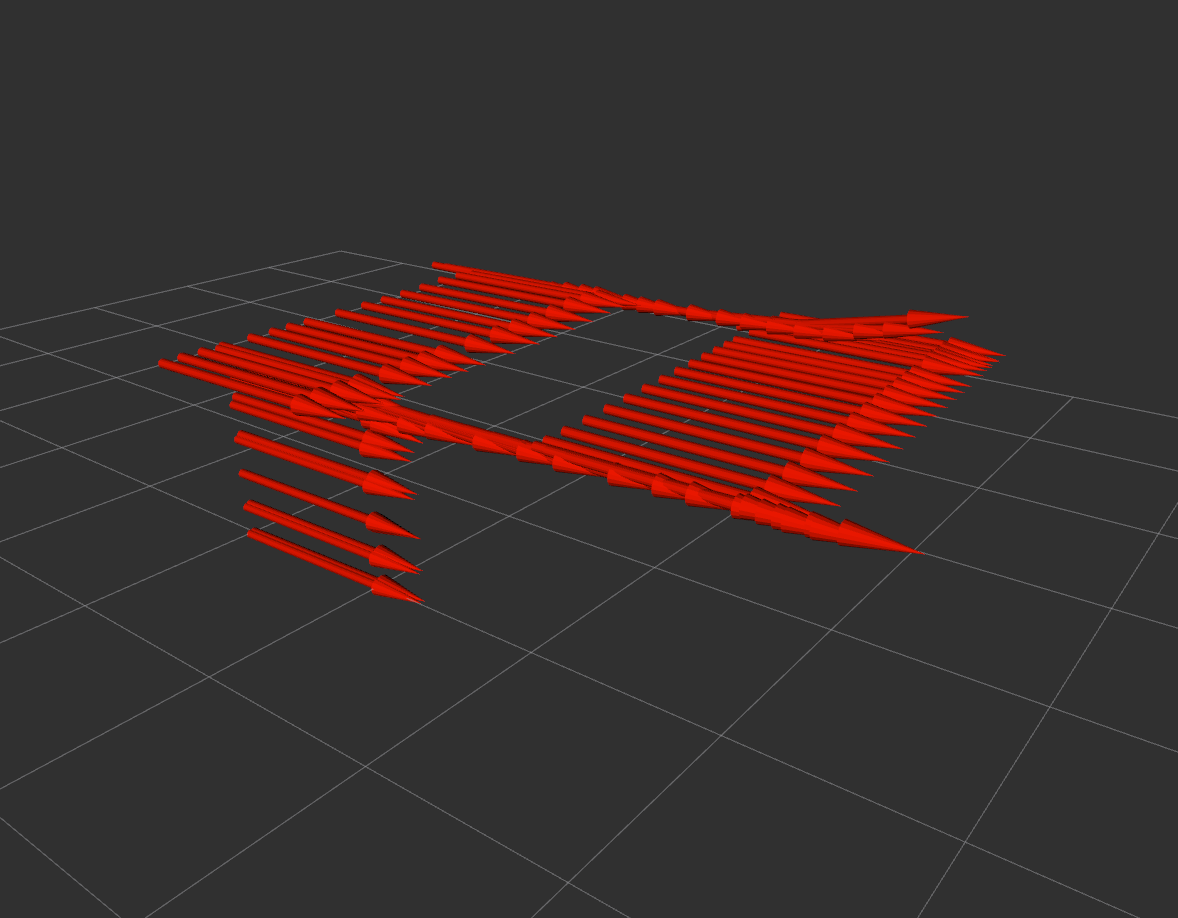
\includegraphics[width=1.0\linewidth]{images/task2_sim_rviz.png}
	\caption{x, y and z coordinates of the drone in simulation. (Kp = 0.1, Ki = 0.01, Kd = 0.1)}
	\label{fig:sim_rviz}
\end{figure}

\subsection{Real world results}
After having tested the controller in simulation the next step is to test it in a real world scenario. This is done using the Vicon motion control system which is able to accurately measure a UAV's position. This is done through 12 motion capture cameras that can locate small grey balls which are taped onto the drone itself. The Vicon system uses these balls as an reference point in space which can then be grouped together in the Vicon software and it will be able to publish the position as a topic in ROS.

\section{Conclusion}
The main objective for this project has been to develop control software for a UAV so it would be able to navigate to four coordinate-points in 3D space. The plots shown during the Results and discussion section have clearly shown how the UAV reaches the four points. Furthermore different tools for analysing the UAV data have been used such as rviz. Task 2 haven't been completed because of time constraints and would have high priority for future work.

\begin{thebibliography}{00}

\bibitem{ros} http://wiki.ros.org/, date: 3/10/2020

\bibitem{Week3} Erdal Kaycan, ``Control Of Mobile Robots, week 3: Ground Robot models``, 16th of September 2020

\bibitem{book} RANDAL W. BEARD and TIMOTHY W. McLAIN, SMALL UNMANNED AIRCRAFT Theory and Practice, 2012

\end{thebibliography}
\vspace{12pt}

\end{document}
